\chapter{Theoretical Background}
\label{sec:chap2}

\section{Artificial Neural Networks}
Artificial neural networks are widely successful in a great number of areas of computer science, often achieving better than human efficiency. This chapter offers a brief introduction to principles of artificial neural networks. For more in depth information we recommend \cite{goodfellow_deep_2016}. Artificial neural networks are parametric models -- parameters are usually called \textit{weights} and are learned during the training of the network. On the other hand \textit{hyperparameters} are parameters whose values are set before the learning process begins. 


\subsection{Feedforward Neural Networks}
\textit{Artificial neural networks} are computing systems inspired by the structure of central nervous system of animals. A basic computing unit of the network is called \textit{neuron}, which performs some simple computation on its inputs and produces its output. Neurons are connected by weighted connections and so create a network. \par
\textit{Feedforward Neural Networks} are networks where the information is only passed in one direction, so the graph of the network is an acyclic directed graph. The simplest network architecture is the so called \textit{Single-layer perceptron}. It consists of a single layer of output neurons; the inputs are fed directly to the outputs via a series of weights. Each neuron can also have a bias value and activation function. Then the output of a neuron is computed: $$output_j = f(\sum_{i \in inputs} {w_{ij}*i + b_j})$$ Where $f$ is an activation function, $w_{ij}$ is a weight of the connection from $i-th$ input neuron to $j-th$ output neuron and $b_j$ is its bias value .

\begin{figure}
\def\layersep{2.5cm}
\centering
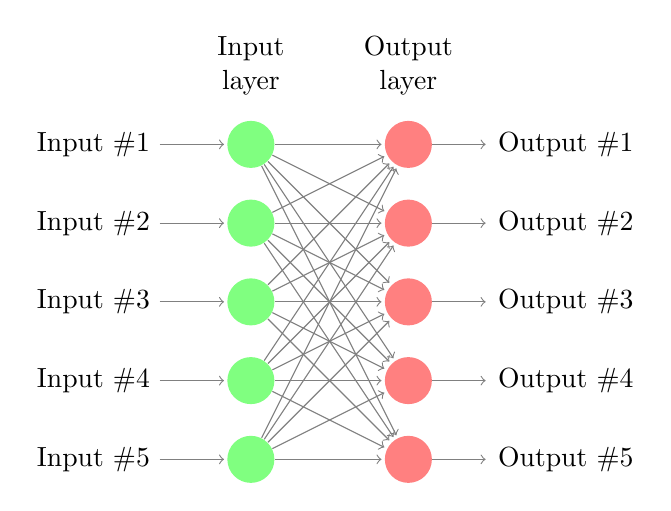
\begin{tikzpicture}[shorten >=1pt,->,draw=black!50, node distance=\layersep]
\tikzstyle{every pin edge}=[<-,shorten <=1pt]
\tikzstyle{neuron}=[circle,fill=black!25,minimum size=17pt,inner sep=0pt]
\tikzstyle{input neuron}=[neuron, fill=green!50];
\tikzstyle{output neuron}=[neuron, fill=red!50];
\tikzstyle{annot} = [text width=4em, text centered]

% Write input labels
\foreach \name / \y in {1,...,5}
\node (IL-\name) at (0,-\y) {Input \#\y};

% Draw the input layer nodes
\foreach \name / \y in {1,...,5}
\node[input neuron, right of=IL-\name] (I-\name) {};

\foreach \source in {1,...,5}
\path (IL-\source) edge (I-\source);

% Draw the hidden layer nodes
\foreach \name / \y in {1,...,5}
\node[output neuron, right of=I-\name] (O-\name) {};

%Write output labels
\foreach \name / \y in {1,...,5}
\node[right of=O-\name] (OL-\name) {Output \#\y};

\foreach \source in {1,...,5}
\path (O-\source) edge (OL-\source);

% Connect every node in the hidden layer with the output layer
\foreach \source in {1,...,5}
\foreach \dest in {1,...,5}
\path (I-\source) edge (O-\dest);

%Annotate the layers
\node[annot,above of=O-1, node distance=1cm] {Output layer};
\node[annot,above of=I-1, node distance=1cm] {Input layer};

\end{tikzpicture}
\caption{Single-layer perceptron}
\label{singlelayerperceptron}
\end{figure}
The activation function can be an arbitrary function but is required to be non-linear and differentiable. Most commonly used are the sigmoid function, hyperbolic tangent and rectified linear unit (ReLU), defined as $ReLU(x) = max(0,x)$.\par  
We can insert one or more layers of neurons between input and output obtaining a \textit{Multi-layered perceptron}. Neuron from $i-th$ layer gets its input from all neurons from $(i-1)-th$ layer and passes its output to all neurons in $(i+1)-th$ layer. Therefore this type of layer is called \textit{fully connected layer} or sometimes dense layer.  We can also rewrite all the weights to a matrix form and obtain the so called weight matrix. Output of a fully connected layer can be expressed as follows: 
$$output_i = f(W_i * output_{i-1} + b_i)$$
Where $f$ is an activation function, $W_i$ is the weight matrix and $b_i$ is a vector of biases.\par  
Multi layered perceptrons can be trained for variety of tasks using a gradient descent algorithm by backpropagating the error of the trained task through the network in direction from outputs to inputs. Fully connected layers are used in almost all other types of neural networks especially as last layers in the network, producing feature vectors or classification distributions.


\begin{figure}
\def\layersep{2.0cm}
\centering
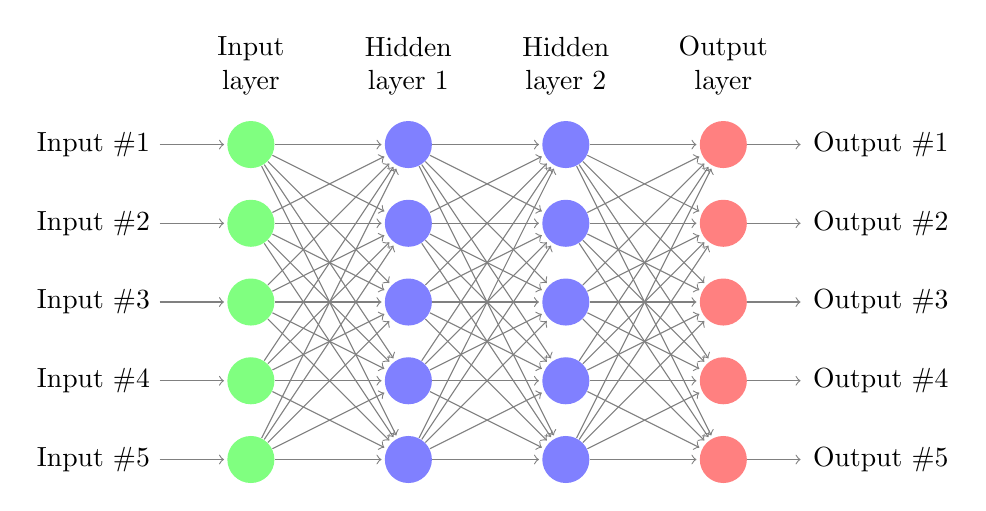
\begin{tikzpicture}[shorten >=1pt,->,draw=black!50, node distance=\layersep]
\tikzstyle{every pin edge}=[<-,shorten <=1pt]
\tikzstyle{neuron}=[circle,fill=black!25,minimum size=17pt,inner sep=0pt]
\tikzstyle{input neuron}=[neuron, fill=green!50];
\tikzstyle{output neuron}=[neuron, fill=red!50];
\tikzstyle{hidden neuron}=[neuron, fill=blue!50];
\tikzstyle{annot} = [text width=4em, text centered]

% Write input labels
\foreach \name / \y in {1,...,5}
\node (IL-\name) at (0,-\y) {Input \#\y};

% Draw the input layer nodes
\foreach \name / \y in {1,...,5}
\node[input neuron, right of=IL-\name] (I-\name) {};

\foreach \source in {1,...,5}
\path (IL-\source) edge (I-\source);

% Draw the hidden layer nodes
\foreach \name / \y in {1,...,5}
\node[hidden neuron, right of=I-\name] (H1-\name) {};

% Draw the hidden layer nodes
\foreach \name / \y in {1,...,5}
\node[hidden neuron, right of=H1-\name] (H2-\name) {};

% Draw the output layer nodes
\foreach \name / \y in {1,...,5}
\node[output neuron, right of=H2-\name] (O-\name) {};

%Write output labels
\foreach \name / \y in {1,...,5}
\node[right of=O-\name] (OL-\name) {Output \#\y};

\foreach \source in {1,...,5}
\path (O-\source) edge (OL-\source);

% Connect every node in the hidden layer with the output layer
\foreach \source in {1,...,5}
\foreach \dest in {1,...,5}
\path (I-\source) edge (H1-\dest);

\foreach \source in {1,...,5}
\foreach \dest in {1,...,5}
\path (H1-\source) edge (H2-\dest);

\foreach \source in {1,...,5}
\foreach \dest in {1,...,5}
\path (H2-\source) edge (O-\dest);

%Annotate the layers
\node[annot,above of=O-1, node distance=1cm] {Output layer};
\node[annot,above of=I-1, node distance=1cm] {Input layer};
\node[annot,above of=H1-1, node distance=1cm] {Hidden layer 1};
\node[annot,above of=H2-1, node distance=1cm] {Hidden layer 2};

\end{tikzpicture}
\caption{Multi-layer perceptron}
\label{multilayerperceptron}
\end{figure}

\subsection{Convolutional Neural Networks}
\textit{Convolutional Neural Networks} (first introduced in \cite{lecun_backpropagation_1989}) are designed to be better in capturing the spatio-temporal data than the standard fully connected layers. They are most successful in processing two-dimensional images so we will describe this case. However, also one-dimensional and three dimensional convolutions are used as shall be described later.  \par
Weights of the convolutional layers are connected to only a small region of the data and shared across the spatio-temporal dimensions. In the case of images this means that the convolutional layer is connected to only small patches of the image and weights are shared among these patches. Weights of the convolutional layers are typically called \textit{filters} or \textit{kernels}. A common approach is to slide the filter across the whole image,  computing local features for each pixel.
Two dimensional convolution can be defined:
$$Conv(i,j) = \sum_m {\sum_n {I(i+m,j+n)K(m,n)}}$$ where $I$ is the input image and $K$ represents the weights of the kernel.\par
The speed of the sliding window is a parameter called \textit{stride}. By having a stride bigger than one we skip some pixels in the input, and obtain an image with smaller width and height. We also need to employ one of the padding schemes on the edges of input image. The most usual type of padding is \textit{zero padding}, which counts areas outside of picture as having value of zero and is preserving original dimensions. Another approach, \textit{valid padding}, is to ignore the edge pixels of the input image altogether, sliding the filter only across valid positions - this produces a smaller output image.
By stacking more convolutional layers atop each other and creating deep convolutional network,  global features of the image can be extracted. 
\par
Another important type of layer used in convolutional neural networks is a pooling layer. It is usually used on the feature maps obtained by convolutional layers. The goal of the pooling is to get some translation invariance in produced features. Similarly to the convolution, pooling also scans the entire input feature map in a sliding-window fashion. However it does not perform convolution but maximum, average or a similar function. Unlike with convolution, stride bigger than one is used when using pooling in order to reduce the size of the output features.
The most commonly used type of pooling -- max pooling -- can be described by the following formula: 
$$maxpool(I)[x,y] =
\max_{\substack{0 \leq i < d_h\\
		0 \leq j < d_w}}
I[x + i - \lfloor \frac{d_h}{2} \rfloor, y + j - \lfloor \frac{d_w}{2}  \rfloor ] $$ Where $x$ and $y$ are coordinates of a pixel in the picture, $d_h$ and $d_w$ are sizes of the sliding window.\par
Convolutional layers are much more efficient than fully connected layers as they share their parameters across the image and have been very successful in variety of image, video and natural language processing tasks. 

\subsection{Recurrent Neural Networks}
Another widely used class of artificial neural networks are \textit{recurrent neural networks}. In contrast to the previously described networks, they take as their input also their previous state representing a kind of memory. Recurrent neural networks are well suited for processing of sequenced data, such as video, text or speech. A typical architecture of RNN is \textit{encoder-decoder} architecture. Encoder produces a feature vector by processing the input sequence. Decoder then constructs an output sequence from the feature vector. To give the network control over its memory, two types of cells were devised: Long short-term memory unit (LSTM) \cite{hochreiter_long_1997} and Gated recurrent unit (GRU) \cite{cho_learning_2014}. Important concept, which leads to better performance, is \textit{attention} \cite{bahdanau_neural_2014} -- it allows the network to learn which parts of the input sequence are important and how they correspond to the output sequence.
Only one of networks we have tested uses recurrent neural networks so we refer to \cite{goodfellow_deep_2016} for further information.

\subsection{Regularization}
Overfitting is a common problem in machine learning. It is a phenomenon when a model represents the training set too well and fails to generalize. To avoid this problem several regularization techniques are employed. We can add regularization directly to the optimized loss function. This is usually implemented by adding some term which keeps the weights of the network in low absolute values. \par
Dropout \cite{srivastava_dropout:_2014} is a stochastic regularization technique; during training, at every iteration, it randomly selects some nodes and removes them along with all of their incoming and outgoing connections. So each iteration has a different set of nodes and this results in a different set of outputs. It is a very effective technique which can be thought of as training a whole ensemble of networks at once. Dropout is usually applied after each fully connected layer. \par
Another common way how to avoid overfitting is by increasing the size of the training set by some data augmentation. Specifics of data augmentation depend on the kind of data we are working with, but in general the dataset is increased by creating new instances from the training dataset. For example with image data, we can use geometric transformations such as mirroring, rotating, translating or scaling. We will see several examples of data augmentation in later chapters.

\subsection{Training}
In recent years very deep (tens of layers) neural networks are used. To train such a network several improvements were developed. Mini-batch training is used almost in all cases. The training dataset is divided into small chunks (typically 32 or 64 examples) and one batch is presented , gradient is computed and weights are updated correspondingly in each step of the training. This is much more efficient than computing gradient of the whole dataset and has some positive regularization effects. \par
For deep networks it is no longer sufficient to use a simple gradient descent algorithm. To speed up and stabilize the training process algorithms with momentum such as Nesterov momentum \cite{sutskever_importance_2013} has been used. 
An important hyperparameter of the network is the learning rate, which controls the speed of training. Set the learning rate too small and network can not learn at all, too big and the weights can diverge. To solve this problem, algorithms with adaptive learning rates, such as 
RMSProp \cite{hinton_neural_nodate} or ADAM \cite{kingma_adam:_2014}, are used. \par
Another obstacle in training is that the information contained in the gradient gets lost in deep neural networks during the backpropagation phase of the algorithm. It either diminishes to zero or grows rapidly and diverges. This can be avoided by a good choice of the activation function (in modern networks mainly ReLU is used) or by some normalization technique. A prime example of this is \textit{batch normalization} \cite{ioffe_batch_2015}, which normalizes the inputs of the layer by subtracting the mean of the batch and dividing by its standard deviation. These changes would be discarded by the learning algorithm, so we add two learnable parameters representing the mean and standard deviation, and the output of the layer is again denormalized using these parameters. This effectively allows the network to learn the correct scaling of the weights using only two parameters instead of changing the whole network, which leads to a much greater stability of the training.\par
Another widely used technique allowing training of very deep networks are \textit{residual connections} \cite{szegedy_inception-v4_2016} A residual connection allows the network to skip the layer and choose to work with the input instead. This makes copying the information through the network possible and helps to reduce the vanishing gradient problem.

\section{Deep Learning Frameworks}
In recent years several software frameworks for machine learning in general and for deep learning in particular are being developed. They are usually implemented in C++ for performance but provide a Python API for more convenient use. All of the following libraries are open-source and publicly available. They also implement support for running the machine learning algorithms on GPU - a key feature for fast training of deep neural networks. \par
One of the most widely used deep learning frameworks is TensorFlow \cite{martin_abadi_tensorflow:_2015} developed by team at Google. It is a symbolic math library and implements all the standard neural layers and also many of the latest developments in the area of deep learning.  \par
PyTorch \cite{paszke_automatic_2017} is a Python extension of a Torch machine learning library. It is primarily developed by Facebook. It focuses on simple usage and Python integration and implements all the standard functions as well as extended tools for various areas of machine learning. \par
Caffe \cite{jia_caffe:_2014} is a deep learning framework originally developed at University of California, Berkeley. It offers good speed and training models without writing any code just network definition. It does not seem to be developing as quickly as above mentioned frameworks. There was also Caffe2 developed by Facebook, but it was merged into PyTorch. \par
Theano \cite{theano_development_team_theano:_2016} is a Python library for manipulating and evaluating mathematical expressions, primarily developed by a Montreal Institute for Learning Algorithms (MILA) at the Université de Montréal. Lasagne \cite{dieleman_lasagne:_2015} is a lightweight library which uses Theano for machine learning computations. It also does not seem to be developing quickly enough at a present. 
Other favourite deep learning frameworks	, which we do not use in our work, include Microsoft Cognitive Toolkit (CNTK) \cite{seide_cntk:_2016} developed by Microsoft and Keras \cite{chollet_keras_2015} which is a high-level API focusing on being user friendly and uses TensorFlow as its backend, but is modifiable to work with other frameworks as well.

